\documentclass[11pt,a4paper]{article}
\usepackage[margin=26mm]{geometry}
\usepackage[T1]{fontenc}
\usepackage{lmodern,microtype,amsmath,amssymb,amsthm,mathtools}
\usepackage{graphicx,booktabs,array,enumitem,xcolor}
\usepackage[hidelinks]{hyperref}
\usepackage{url}
\usepackage{fancyhdr}
\setlength{\headheight}{14pt}
\pagestyle{fancy}
\fancyhf{}\fancyhead[L]{\small Homothetic toroidal models}\fancyhead[R]{\small Candidate v0.1.1}
\fancyfoot[C]{\thepage}
\setlength{\emergencystretch}{2em}
\setlength{\parskip}{3pt}
\renewcommand{\topfraction}{0.9}
\renewcommand{\bottomfraction}{0.85}
\renewcommand{\textfraction}{0.06}
\setlist{nosep}
\newtheorem{theorem}{Theorem}[section]
\newtheorem{proposition}[theorem]{Proposition}
\newtheorem{corollary}[theorem]{Corollary}
\theoremstyle{definition}
\newtheorem{definition}[theorem]{Definition}
\theoremstyle{remark}
\newtheorem{remark}[theorem]{Remark}
\newcommand{\R}{\mathbb R}
\newcommand{\C}{\mathbb C}
\newcommand{\T}{\mathbb T}
\newcommand{\e}{\mathrm e}
\newcommand{\ii}{\mathrm i}
\newcommand{\dd}{\,\mathrm d}
\newcommand{\Rea}{\operatorname{Re}}
\newcommand{\Ima}{\operatorname{Im}}
\newcommand{\atan}{\operatorname{atan2}}
\newcommand{\supp}{\operatorname{supp}}
\DeclareMathOperator{\interior}{int}
\title{\textbf{Homothetic Toroidal Models}\\[3pt]
Geometry, Phase Reconstruction, and Display Information}
\author{Hilmir Frímann Halldórsson}
\date{9 October 2026\\[3pt]\small Version 0.1.1 --- revised repository-research candidate}
\begin{document}
\maketitle
\begin{abstract}
A toroidal formula can specify a surface, an observation on a parameter
domain, or a display of recorded data. We study these meanings separately
for a finite homothetic family of toroidal charts and a prescribed
Gaussian-weighted phase sum. We obtain an exact criterion for intersection
of the full surface images, and distinguish it from strict containment of
associated diagnostic spindle bodies. The squared modulus of the phase
sum depends on the prescribed phase through a span of dimension at most
three, $\operatorname{span}\{1,\cos(2\Phi),\sin(2\Phi)\}$, and is
recovered from three known phase samples under a sharp nonsingularity
condition. A reflection and
exponential-independence argument excludes nonzero rigid azimuthal
rotation under explicit ring-family hypotheses. We derive the induced
area measures, identify their normalization rules, and exhibit
nonunique ambient extensions of the reference-shell observation.
Finally, exact inverses and exceptional fibres characterize three
separate display maps, including the difference between coordinates and
a richer retained record. The results are mathematical consequences of
stated definitions; they do not supply an evolution law or a physical
interpretation. Coordinate-based figures and isolated algebraic and
numerical checks accompany the written proofs.
\end{abstract}

\section{Question, definitions, and scope}
\label{sec:intro}
What geometry and information are determined by a scaled toroidal
construction? A useful answer requires distinguishing the domain of a
formula from its image, and an observation from a display of that
observation. This paper develops that distinction for one finite family
whose radii form geometric progressions. It then analyzes the phase
dependence of a scalar observation and the information retained by
separate coordinate displays. Each construction is defined here, so the
arguments do not require access to historical documents or software.

The geometric starting point is classical: a circle rotated about an
axis produces ring, horn, or spindle images according to the ratio of
its major and minor radii \cite{weissteinTorus}. Circle-intersection
algebra is also classical \cite{weissteinCircles}. The contribution of
Sections~\ref{sec:carriers}--\ref{sec:intersections} is their application
to a fixed-aspect homothetic family, with both signed meridian branches
retained. Sections~\ref{sec:phase}--\ref{sec:rotation} give a finite
phase reduction and a restricted rotation obstruction.
Three-sample recovery is an elementary instance of trigonometric
interpolation; it is related in method, but not identical in sampling
protocol, to phase-shifting reconstruction \cite{chengWyant}.
Sections~\ref{sec:measures}--\ref{sec:displays} concern measures,
extension freedom, and exact inverses of explicitly defined maps.
We make no claim of priority for the underlying geometry or
interpolation principles.

The historical motivation is the common-angle toroidal sum in
\emph{Converging Symmetries} \cite{cs1,cs2} and its later presentation in
\emph{Recursive Field Collapse into Toroidal Attractor Structures}
\cite{rt}. These sources and separate display code motivated the
questions, but do not identify all of their objects with one another.
The short source correspondence in Appendix~\ref{app:sources} records
the limited connection. The present exposition incorporates the final
reconciled reference and subsequent accepted qualifications
\cite{reconciled,addendum,refinements}.

Throughout, $N\geq1$ is a finite integer, $s>1$, and $r_0,R_*>0$.
Indices satisfy $0\leq n<N$. Angles belong to
$\T^2=(\R/2\pi\mathbb Z)^2$. Define
\begin{equation}
 r_n=r_0s^n,\qquad R_n=R_*s^{n-N/2},\qquad
 \bar R=R_*s^{-N/2}=R_{n=0},\qquad a=\frac{\bar R}{r_0}.
 \label{eq:radii}
\end{equation}
The letters $R_n$ and $r_n$ denote geometric radii; $C$ below is an
independent Gaussian-centre parameter. No equality between $C$ and
$R_*$ is assumed. Spatial coordinates are Euclidean. If a length unit
is assigned, all radii and $C$ have that unit and Gaussian precision
$\alpha$ has inverse-square length units. The source does not determine
a physical unit for the complex amplitude or its squared modulus.
Angles and their trigonometric arguments are dimensionless.

The central distinctions can be stated before the proofs. A chart
$X_n:\T^2\to\R^3$ has a full image $S_n$. A body $K_n$, introduced later,
is a separate diagnostic construction. An observation $\psi$ is
initially a function on the common angle domain; its nonnegative
squared modulus $P$ becomes a normalized density only after a measure
and a positive integral are specified. A display map acts on other
recorded quantities and may discard information. Reusing a toroidal
coordinate expression does not provide a mathematical identification
between these objects.

\section{Carriers: homothety and singular charts}
\label{sec:carriers}
Define
\begin{equation}
 X_n(\theta,\phi)=
 \bigl((R_n+r_n\cos\theta)\cos\phi,\,
       (R_n+r_n\cos\theta)\sin\phi,\,
       r_n\sin\theta\bigr),\qquad S_n=X_n(\T^2).
 \label{eq:chart}
\end{equation}
The abstract torus $\T^2$ is always a smooth parameter domain.
Whether \eqref{eq:chart} is an embedding is a different question.

\begin{proposition}[Common aspect and chart classification]
\label{prop:homothety}
Let $Y=X_0$ with major radius $\bar R$ and minor radius $r_0$.
Then $X_n=s^nY$ and $R_n/r_n=a$ for every admissible $n$.
If $a>1$, each chart is an embedding and $S_n$ is a ring torus.
For $a=1$ the chart is noninjective and loses rank along
$\theta=\pi$. For $0<a<1$ it is noninjective and loses rank along
the two parameter circles $\cos\theta=-a$.
\end{proposition}
\begin{proof}
Substitution of \eqref{eq:radii} into each component of
\eqref{eq:chart} factors out $s^n$. Write
$q=R_n+r_n\cos\theta$. Direct differentiation gives
\begin{equation}
 |X_{n,\theta}|^2=r_n^2,\qquad
 X_{n,\theta}\cdot X_{n,\phi}=0,\qquad
 |X_{n,\phi}|^2=q^2.
 \label{eq:metric}
\end{equation}
For a ring, $q>0$. The spatial cylindrical radius
$\rho=\sqrt{x^2+y^2}$ equals $q$, and the point determines
$\phi=\atan(y,x)$ and
$\theta=\atan(z,\rho-R_n)$ modulo $2\pi$. Thus the chart is
injective and has rank two. A continuous injection from the compact
domain into the Hausdorff space $\R^3$ is a homeomorphism onto its
image, proving that this immersion is an embedding.

For a horn, $q=0$ exactly at $\theta=\pi$. Every value of $\phi$
there maps to the origin, and $X_{n,\phi}=0$ while
$|X_{n,\theta}|=r_n>0$. For a spindle, $q=0$ at two values of
$\theta$, with respective heights
$z=\pm r_n\sqrt{1-a^2}$. Each entire parameter circle collapses
to one of these axis points, and the rank is again one there.
These collapses establish noninjectivity without requiring a
classification of every fibre elsewhere.
\end{proof}

The family has one aspect ratio, not a succession of different
ring/horn/spindle types. Holding $R_*/r_0$ and $s$ fixed, the equation
for a horn is
\begin{equation}
 N=\frac{2\log(R_*/r_0)}{\log s}.
 \label{eq:hornN}
\end{equation}
It determines an admissible model only if the right side is a positive
integer. It need not be one. Statements comparing two shells also
require $N\geq2$ and valid indices; an arbitrary real solution of
\eqref{eq:hornN} supplies neither condition.

For fixed common angles, every $X_n$ lies on the ray through $Y$.
Two different indices give the same point at these angles only when
$Y=0$, which occurs precisely at the horn collapse. This observation
does \emph{not} decide whether the full images intersect: two charts
can reach the same spatial point at different angles. The next section
treats that question.

\begin{figure}[tb]
\centering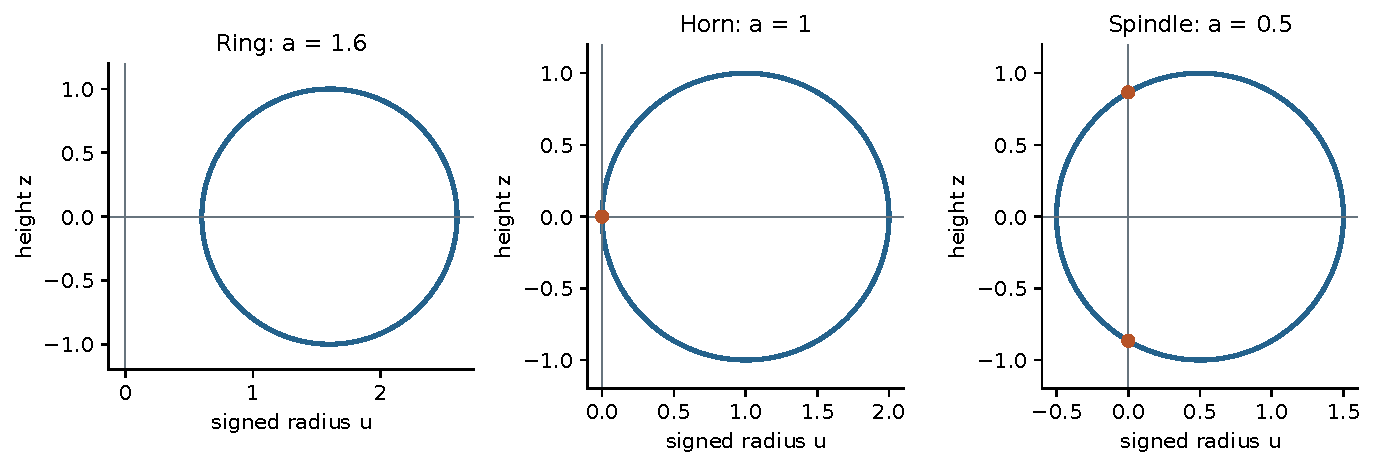
\includegraphics[width=\linewidth]{figures/carriers.pdf}
\caption{Signed meridian charts $(u,z)=(a+\cos\theta,\sin\theta)$
at minor radius one. The vertical line is the axis of revolution.
Ring, horn, and spindle cases use the declared illustrative aspects
$a=1.6,1,0.5$. Rotation uses the signed coordinate $u$; negative
$u$ is not to be discarded when forming the full image.}
\label{fig:carriers}
\end{figure}

\section{Image intersection and a separate body diagnostic}
\label{sec:intersections}
\subsection{The full-image criterion}
Fix admissible indices $n,n+k$ with $k\geq1$ and $n+k<N$.
Put $r=r_n$ and $h=s^k>1$. The second shell has radii
$(ahr,hr)$ while the first has radii $(ar,r)$.

\begin{theorem}[Intersection of full images]
\label{thm:intersection}
The two surface images meet if and only if
\begin{equation}
 L(h):=\frac{h-1}{h+1}\ \leq a\leq\
 U(h):=\frac{h+1}{h-1}.
 \label{eq:intersection}
\end{equation}
The endpoints are tangencies of the appropriate meridian circles.
For $a=1$, the two images meet only at the origin.
\end{theorem}
\begin{proof}
In a signed meridian plane use coordinates $(u,z)$ and the circle
\[
 (u-ar)^2+z^2=r^2.
\]
Rotation about the $z$ axis maps $u$ and $-u$ to the same cylindrical
radius. Consequently a spatial point can be on both images either
from two same-side meridian circles or from one circle and the
reflection of the other. This covers every case: for any common point,
each signed radius is one of $\rho,-\rho$, where
$\rho=\sqrt{x^2+y^2}$; a common reflection makes the first sign
positive or negative as needed, leaving only those two comparisons.

For completeness, two circles of radii $r$ and $hr$, whose centres
are separated by $d>0$, meet precisely when
$(h-1)r\leq d\leq(h+1)r$. To see sufficiency as well as necessity,
place their centres at $(0,0)$ and $(d,0)$. Subtracting the circle
equations gives
\[
 u_*=\frac{d^2+r^2-h^2r^2}{2d},\qquad
 z_*^2=r^2-u_*^2
 =\frac{\bigl((h+1)^2r^2-d^2\bigr)
             \bigl(d^2-(h-1)^2r^2\bigr)}{4d^2}.
\]
The last expression is nonnegative exactly on the stated interval;
then $(u_*,\pm\sqrt{z_*^2})$ supplies the intersection. The same
inequalities are the triangle inequalities for a common point.
Equality gives tangency. This is the usual circle calculation
\cite{weissteinCircles}.

The same-side centres have separation $d=a(h-1)r$, so this case
occurs exactly for $1\leq a\leq U(h)$. Reflecting the second
circle gives separation $d=a(h+1)r$, hence
$L(h)\leq a\leq1$. Their union is \eqref{eq:intersection}.
Rotating a meridian intersection gives a spatial one, so neither
branch is merely a necessary condition.

At $a=1$ the same-side circles are internally tangent at the origin;
the reflected pair is externally tangent there. Thus the origin
is the only common spatial point. At $a=L(h)$ the reflected
circles are internally tangent, and at $a=U(h)$ the same-side
circles are externally tangent. These latter tangent points have
nonzero cylindrical radius, so each rotates into a common circle
in three dimensions.
\end{proof}

In particular, ignoring the reflected circle removes the entire
spindle portion $L(h)\leq a<1$. Counting same-angle coincidences
removes almost all intersections instead. The theorem concerns
sets $S_n$, including their singular images, and makes no statement
about an overlap volume or a dynamical interaction.

\begin{figure}[tb]
\centering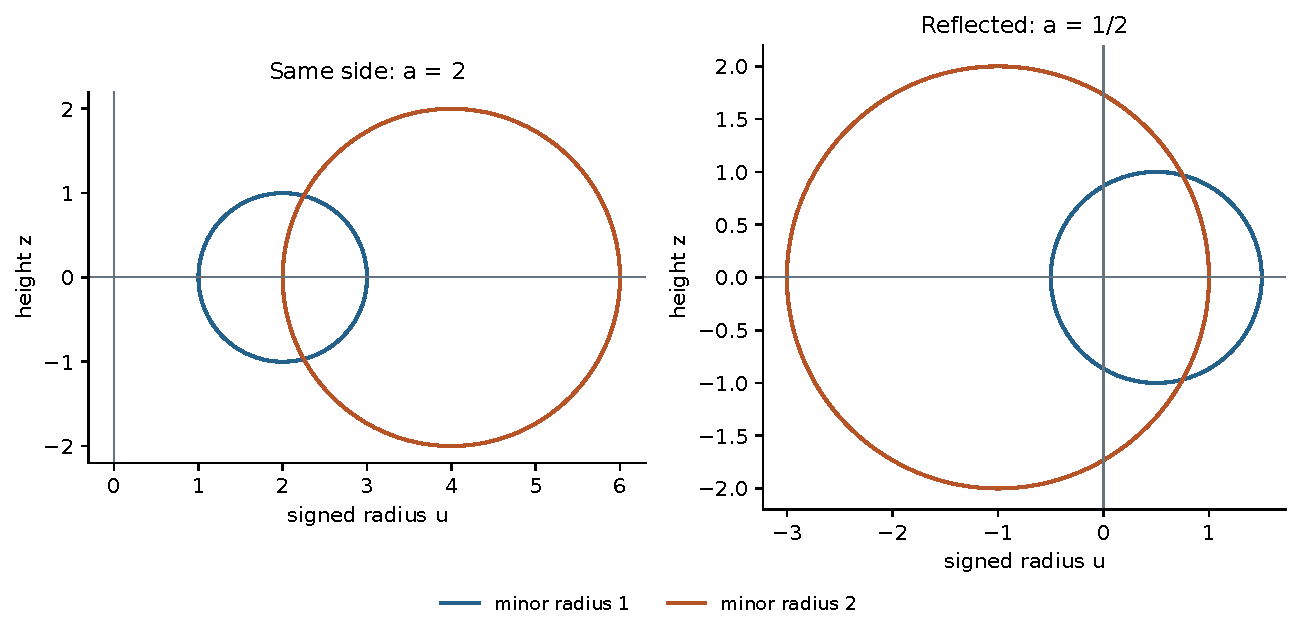
\includegraphics[width=\linewidth]{figures/intersections.pdf}
\caption{Meridian comparisons at $r=1$, $h=2$.
Left: $a=2$ uses same-side circles. Right: $a=1/2$ uses the
reflection of the larger circle. Both lie in the exact interval
$[1/3,3]$. The reflected signed coordinate is a geometric device
for testing full spatial images, not an additional shell.}
\label{fig:intersections}
\end{figure}

\subsection{Strict containment of diagnostic spindle bodies}
Define the closed set
\begin{equation}
 K_n=\{(x,y,z)\in\R^3:
       (\sqrt{x^2+y^2}-R_n)^2+z^2\leq r_n^2\}.
 \label{eq:body}
\end{equation}
This is a chosen diagnostic body. We do not adopt it as a recovered
material region or attach a physical density to its volume.

\begin{theorem}[Containment despite intersecting images]
\label{thm:body}
If $0<a<1$ and $m>n$, then $K_n\subset\interior K_m$.
Writing $\Delta r=r_m-r_n$, the defining radial distance has a
strict margin at least $(1-a)\Delta r>0$. Furthermore
$S_n\subset K_n$, but the spindle portion with
$q=R_n+r_n\cos\theta<0$ lies in the interior of $K_n$ rather than
on its boundary.
\end{theorem}
\begin{proof}
For any point let $v_n=(\rho-ar_n,z)$, where
$\rho=\sqrt{x^2+y^2}\geq0$. If the point is in $K_n$, the triangle
inequality gives
\[
 |v_m|\leq |v_n|+a\Delta r
 \leq r_n+a\Delta r
 =r_m-(1-a)\Delta r<r_m.
\]
Continuity of the defining distance makes this point interior to
$K_m$. This proof applies to every point in the body, including
axis points.

On the chart, $\rho=|q|$ and $z=r_n\sin\theta$. If $q\geq0$,
$(\rho-R_n)^2+z^2=r_n^2$. If $q<0$, expansion instead gives
\begin{equation}
 (\rho-R_n)^2+z^2=r_n^2+4R_nq<r_n^2.
 \label{eq:innersheet}
\end{equation}
Thus all of $S_n$ is in $K_n$, but its negative-$q$ sheet is
interior. The positive-$q$ sheet, with the seams $q=0$, is exactly
the boundary of $K_n$: equality in \eqref{eq:body} reconstructs
$\cos\theta=(\rho-R_n)/r_n$, $\sin\theta=z/r_n$ and $q=\rho$.
At the spindle axis seams, arbitrarily small vertical changes
reach both sides of the defining inequality, so they too are
boundary points.
\end{proof}

Here is an exact witness that makes the distinction concrete. Take
$a=1/2$ and minor radii $1,2$. Then
\begin{equation}
 p=\left(\frac34,0,\frac{\sqrt{15}}4\right)
 \label{eq:witness}
\end{equation}
is on both images. For the small chart choose
$\cos\theta=1/4$, $\sin\theta=\sqrt{15}/4$, $\phi=0$.
For the large chart choose
$\cos\theta=-7/8$, $\sin\theta=\sqrt{15}/8$, $\phi=\pi$.
The large chart has $q=-3/4$, hence its spatial $x$ is $3/4$.
The squared distance in \eqref{eq:body} for the larger body is
$(3/4-1)^2+15/16=1<4$. The point is therefore on the smaller
boundary, on the larger inner image sheet, and strictly inside
the larger body.

The containment proof does not use $L(h)$, and remains valid below
that image-intersection threshold. At $a=1$ the same inequality
only gives nonstrict containment and the common origin is a
boundary point. The strict spindle margin, not the lower
intersection threshold, is what establishes the theorem.

\begin{figure}[tb]
\centering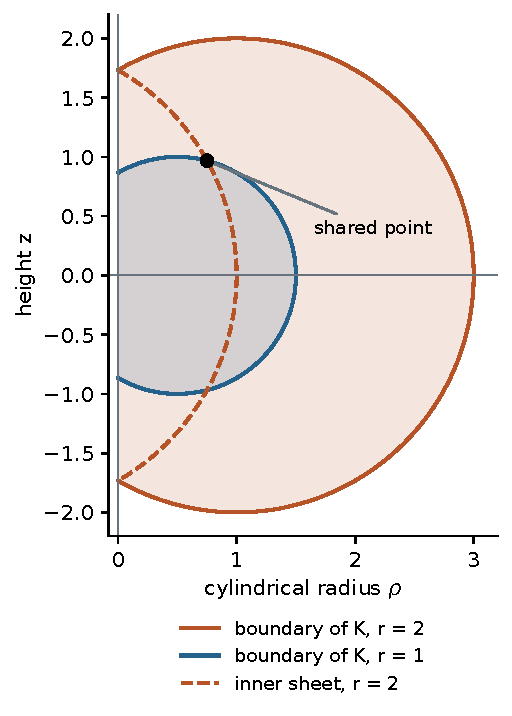
\includegraphics[width=.65\linewidth]{figures/bodies.pdf}
\caption{Physical meridian half-plane $\rho\geq0$ for the exact
witness \eqref{eq:witness}. Shaded sections are the diagnostic
bodies for $a=1/2$, $r=1,2$. The dashed curve is the larger
negative-signed-radius image sheet, folded to $\rho\geq0$.
The marked point lies on that sheet inside the larger body.}
\label{fig:bodies}
\end{figure}

\subsection{A comparison with fixed aspect}
For adjacent shells with $s=\varphi_g=(1+\sqrt5)/2$,
\[
 L(\varphi_g)=\varphi_g^{-3},\qquad
 U(\varphi_g)=\varphi_g^3.
\]
As $h>1$ increases, $L(h)$ increases and $U(h)$ decreases.
Thus, among adjacent scale choices $\varphi_g<\e<\pi$, the
golden-ratio choice has the widest interval of intersecting
\emph{aspects}. For example, at fixed $a=3$ and $N\geq2$,
adjacent golden-ratio shells meet, whereas the choices $\e$ and
$\pi$ do not. This compares the criterion, not intersection
volume, constructive interference, or stability. Holding
$R_*/r_0$ and $N$ fixed instead changes
$a=(R_*/r_0)s^{-N/2}$ when $s$ changes, so it is a different
comparison.

\section{A prescribed phase family}
\label{sec:phase}
\subsection{Domain and finite harmonic reduction}
Fix $\alpha>0$, a real $C$, complex amplitudes $A_n$, and real
shell phases $b_n$. Let $\Phi(t)$ be a prescribed real phase.
No differential equation for $\Phi$ is supplied. The source
choice $b_n=\beta n$ is a special case. Define functions on the
common angle domain by
\begin{align}
 D_n(\theta,\phi)&=|X_n(\theta,\phi)-C e_1|^2 \notag\\
 &=R_n^2+r_n^2+C^2+2R_nr_n\cos\theta
      -2C(R_n+r_n\cos\theta)\cos\phi, \label{eq:D}\\
 w_n(\theta,\phi)&=A_n\e^{-\alpha D_n(\theta,\phi)}, \notag\\
 \psi(\theta,\phi;t)&=\sum_{n=0}^{N-1}
                 w_n(\theta,\phi)\cos(\Phi(t)+b_n),\qquad
 P=|\psi|^2. \label{eq:psi}
\end{align}
Here $e_1=(1,0,0)$. The summands are evaluated at different
spatial shell points sharing the same angles. Thus
\eqref{eq:psi} defines a common-domain sum, not yet a spatial
superposition at one common ambient point.

\begin{theorem}[Three-coefficient phase law]
\label{thm:phase}
Define the fixed complex functions
\[
 U=\sum_n w_n\cos b_n,\qquad V=\sum_n w_n\sin b_n.
\]
For a free phase value $\Phi$,
\begin{align}
 \psi&=U\cos\Phi-V\sin\Phi, \label{eq:UV}\\
 P(\Phi)&=c_0+c_1\cos(2\Phi)+c_2\sin(2\Phi), \label{eq:three}\\
 c_0&=\tfrac12(|U|^2+|V|^2),\quad
 c_1=\tfrac12(|U|^2-|V|^2),\quad
 c_2=-\Rea(U\overline V). \label{eq:coeff}
\end{align}
The real linear span of the phase-indexed functions $P(\Phi)$
has dimension at most three, and $P$ is $\pi$-periodic as a
function of $\Phi$.
\end{theorem}
\begin{proof}
The addition law for $\cos(\Phi+b_n)$ gives \eqref{eq:UV}.
Multiplication by its complex conjugate gives
\[
 |\psi|^2=|U|^2\cos^2\Phi+|V|^2\sin^2\Phi
       -2\Rea(U\overline V)\sin\Phi\cos\Phi.
\]
The double-angle identities yield \eqref{eq:three} and
\eqref{eq:coeff}. Every density in the family is a real
linear combination of the three fixed functions $c_0,c_1,c_2$;
these need not be independent. The stated phase period follows
from the doubled arguments.
\end{proof}

Phase periodicity says nothing by itself about periodicity in
$t$. For example, a phase that scans nonuniformly need not
give a periodic time trace. Nor does the rank-three observation
supply an evolution equation for amplitudes or radii.

\begin{proposition}[Modulation and zeros]
\label{prop:modulation}
Pointwise on $\T^2$,
\begin{equation}
 c_0^2-c_1^2-c_2^2=\bigl(\Ima(U\overline V)\bigr)^2.
 \label{eq:modulation}
\end{equation}
Consequently $M=(c_1^2+c_2^2)^{1/2}\leq c_0$ and the range of
$P$ as $\Phi$ varies is $[c_0-M,c_0+M]$. If $U,V$ are real
and not both zero at a point, there is one zero phase modulo
$\pi$. If both vanish, all phases vanish there.
\end{proposition}
\begin{proof}
Subtracting the first two squared coefficients gives
$c_0^2-c_1^2=|U|^2|V|^2=|U\overline V|^2$; subtracting
$c_2^2$ leaves the squared imaginary part. Nonnegativity of
$c_0$ proves the bound. The sinusoid
$c_1\cos2\Phi+c_2\sin2\Phi$ has range $[-M,M]$, including
the constant case $M=0$.

For real $U,V$ put $B=\sqrt{U^2+V^2}>0$ and choose
$\delta$ with $(U,V)=B(\cos\delta,\sin\delta)$. Then
$P=B^2\cos^2(\Phi+\delta)$, which has exactly one zero
modulo $\pi$. The case $B=0$ is immediate.
\end{proof}

For general complex pairs the density may be strictly positive
at every phase. It is constant precisely when $c_1=c_2=0$.
Pointwise zeros at different phases must not be mistaken for
a simultaneous zero of the whole pattern. A useful simultaneous
case is $N=1$: when $\cos(\Phi+b_0)=0$, the entire pattern
vanishes, for any $A_0$. If $A_0=0$ it vanishes at every phase.
These are exact blink cases, relevant to normalization below.

\subsection{Three samples and what they recover}
\begin{theorem}[Known-phase reconstruction]
\label{thm:reconstruction}
At each point, let $P_0,P_{45},P_{90}$ be the intensities at
phases $0,\pi/4,\pi/2$, respectively. Then
\begin{equation}
 c_0=\frac{P_0+P_{90}}2,\qquad
 c_1=\frac{P_0-P_{90}}2,\qquad
 c_2=P_{45}-c_0.
 \label{eq:threeinverse}
\end{equation}
For three arbitrary known phases $\Phi_a,\Phi_b,\Phi_c$ the
coefficient matrix with rows $(1,\cos2\Phi_j,\sin2\Phi_j)$ has
determinant
\begin{equation}
 4\sin(\Phi_b-\Phi_a)\sin(\Phi_c-\Phi_b)
       \sin(\Phi_c-\Phi_a).
 \label{eq:det}
\end{equation}
Hence unrestricted coefficient triples are uniquely recovered
exactly when the known phases are pairwise distinct modulo $\pi$.
\end{theorem}
\begin{proof}
At the three specified phases the rows are $(1,1,0)$,
$(1,0,1)$, and $(1,-1,0)$, giving \eqref{eq:threeinverse}.
For the determinant, subtract row $a$ from rows $b,c$.
The difference pair for a phase $v$ relative to $u$ is
\[
 (\cos2v-\cos2u,\sin2v-\sin2u)
 =2\sin(v-u)(-\sin(v+u),\cos(v+u)).
 \]
Factoring the two sine factors from the remaining $2$ by $2$
determinant leaves $\sin(\Phi_c-\Phi_b)$. This yields
\eqref{eq:det}. The matrix is invertible exactly when all
three factors are nonzero. If it is singular, adding any
nonzero null vector to a coefficient triple leaves the sampled
values unchanged; there is no general linear uniqueness.
\end{proof}

The theorem determines the complete phase-indexed density
\eqref{eq:three}, not the complex amplitude, a phase history,
or the individual shell coefficients. It is a known-phase
result. Phase-shifting interferometry also recovers quantities
from intensities at several shifts \cite[Sec.~I]{chengWyant},
but its experimental interpretation and calibration procedures
are not assumed here. In particular, our doubled sample phases
are $0,\pi/2,\pi$, rather than the equal $120^\circ$ shifts
of the three-bucket procedure discussed by Cheng and Wyant
\cite[Sec.~III.C]{chengWyant}.

Exact uniqueness also differs from numerical conditioning.
As two phases approach congruence modulo $\pi$, the matrix
approaches a singular matrix. Its inverse sensitivity can
therefore become large; the condition number depends on the
chosen norm and error model \cite{higham}. We neither optimize
sample phases nor assert a noise bound. Figure~\ref{fig:phase}
illustrates the exact reconstruction for one declared example.

\begin{figure}[tb]
\centering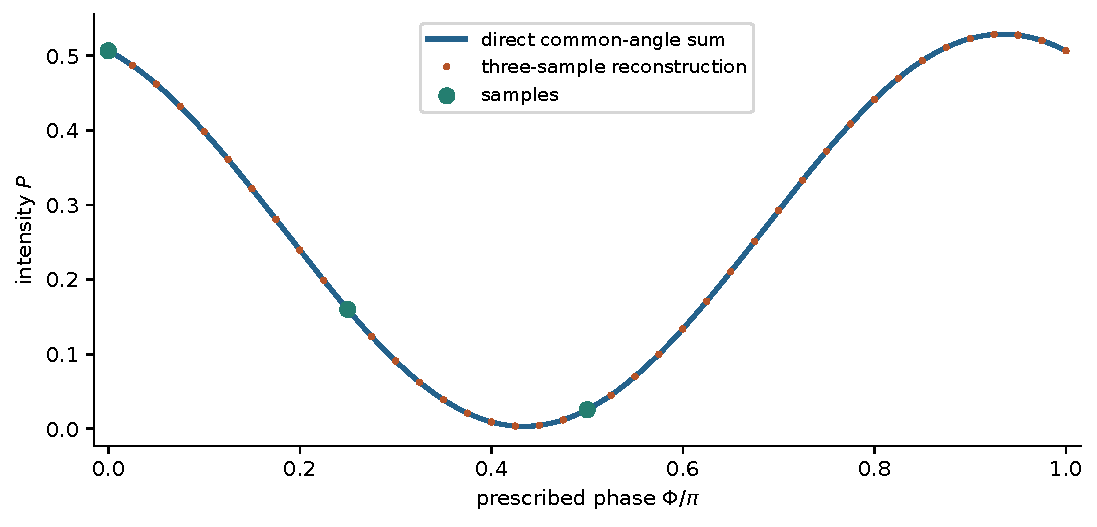
\includegraphics[width=.91\linewidth]{figures/phase.pdf}
\caption{Three-phase recovery at one common-angle point of a
ring-family example. Parameters are $N=3$, $s=1.5$, $r_0=1$,
$a=2$, $C=1$, $\alpha=0.08$,
$A=(1,0.7\e^{0.6\ii},0.4\e^{-0.4\ii})$,
$b=(0,0.8,1.7)$ and $(\theta,\phi)=(0.7,1.1)$.
The curve computed from the source sum coincides with the
reconstruction from the three marked samples. This is a
prescribed phase scan, not a simulated time evolution.}
\label{fig:phase}
\end{figure}

For the abstract reduction \eqref{eq:UV}, the pairs
$(U,V)=(1,\ii)$ and $(1,-\ii)$ produce
$\psi=\e^{-\ii\Phi}$ and $\e^{\ii\Phi}$, respectively.
Both give $P=1$. This is an amplitude-pair nonuniqueness witness;
we do not claim that these constant pairs are realized by a
nonzero restricted Gaussian ring family.
A direct ambiguity \emph{within} that family is
$A_n\mapsto\e^{\ii\delta}A_n$ for every $n$, which multiplies
$\psi$ by an overall phase and leaves $P$ unchanged.
No unique per-shell recovery follows from three density samples.

\section{A restricted obstruction to rigid rotation}
\label{sec:rotation}
A varying threshold picture can appear to move without being a
rigidly rotated fixed pattern. We now give a precise test for the
latter notion. The hypotheses matter: the result below is for
the finite family \eqref{eq:psi}, fixed coefficients, ring
geometry, and a positive off-axis Gaussian centre.

\par\noindent\begin{minipage}{\linewidth}
\begin{theorem}[No nonzero continuously rotating rigid profile]
\label{thm:rotation}
Assume $s>1$, $a>1$, $C>0$, $\alpha>0$, finite $N\geq1$, and
fixed $A_n\in\C$, $b_n\in\R$. Let $I$ be an interval and
$\gamma:I\to\R$ a continuous nonconstant function. Suppose
there exists one fixed function $H$ on $\T^2$ such that
\begin{equation}
 P(\theta,\phi;t)=H(\theta,\phi-\gamma(t))
 \quad\hbox{for every }(\theta,\phi)\in\T^2,\ t\in I.
 \label{eq:rotation}
\end{equation}
Then $P$ is identically zero on $\T^2\times I$. In fact,
$A_n\cos(\Phi(t)+b_n)=0$ for every $n,t$.
\end{theorem}
\end{minipage}\par
\begin{proof}
Equation~\eqref{eq:D} depends on $\phi$ only through
$\cos\phi$. Thus $P(\theta,\phi;t)=P(\theta,-\phi;t)$.
Substituting \eqref{eq:rotation}, and putting
$x=\phi-\gamma(t)$, gives
\[
 H(\theta,x)=H(\theta,-x-2\gamma(t)).
\]
Composing the reflections for two times shows that $H$ has
every angular period $2(\gamma(t)-\gamma(u))$, with either
sign immaterial. Since a continuous nonconstant real function
on an interval has an image containing a nondegenerate interval,
these differences contain a neighborhood of zero. Invariance
under all sufficiently small translations implies invariance
under every translation: express any real displacement as an
integer multiple of a sufficiently small one. Therefore $H$,
and hence each $P(\cdot,\cdot;t)$, is independent of $\phi$.

It remains to exclude a nonzero axisymmetric member of this
family. Fix $\theta=0$ and a time $t$. With $Y=Y(0,\phi)$,
the norm $|Y|^2=(\bar R+r_0)^2$ is independent of $\phi$.
The amplitude takes the form
\begin{equation}
 \psi(0,\phi;t)=\sum_{n=0}^{N-1} d_n(t)\e^{\lambda_n\cos\phi},
 \quad
 \begin{cases}
 d_n=A_n\cos(\Phi(t)+b_n)
       \e^{-\alpha(s^{2n}(\bar R+r_0)^2+C^2)},\\
 \lambda_n=2\alpha C s^n(\bar R+r_0).
 \end{cases}
 \label{eq:exponential}
\end{equation}
The $\lambda_n$ are positive and strictly increasing. Put
$x=\cos\phi$. Axisymmetry implies that
\begin{equation}
 \sum_{n,m}d_n\overline{d_m}\e^{(\lambda_n+\lambda_m)x}
       -K=0\qquad(-1\leq x\leq1)
 \label{eq:expconstant}
\end{equation}
for some real constant $K\geq0$.

Distinct real exponentials are linearly independent on this
interval. Indeed, for distinct exponents $\mu_1,\ldots,\mu_\ell$,
differentiate a zero combination $0,\ldots,\ell-1$ times at an
interior point. After factoring the nonzero
$\e^{\mu_jx}$ from columns, the matrix is Vandermonde, with
determinant $\prod_{i<j}(\mu_j-\mu_i)\neq0$. All coefficients
must vanish.

If any $d_n\neq0$, let $L$ be the largest such index. Among
all terms with nonzero coefficients in \eqref{eq:expconstant},
the largest exponent is $2\lambda_L$. It arises uniquely from
$(n,m)=(L,L)$ and has coefficient $|d_L|^2>0$.
Mixed sums can coincide with one another, but none reaches this
extreme diagonal exponent. The constant term has exponent zero,
strictly smaller than $2\lambda_L$. Grouping coincident lower
exponents and applying independence gives a contradiction.
Thus every $d_n=0$. The Gaussian factors in
\eqref{eq:exponential} are positive, so
$A_n\cos(\Phi(t)+b_n)=0$ for each $n$. This holds at every
$t$, and \eqref{eq:psi} then vanishes at every angle.
\end{proof}

The proof is analytic; checking sampled azimuths could not
establish its conclusion. It does not require that $\Phi$
itself be continuous or nonconstant. A phase held at a complete
blink is a possible zero family, even when some $A_n\neq0$.
The conclusion is therefore zero \emph{pattern}, not necessarily
zero fixed coefficients.

The theorem does not address a centred choice $C=0$, a phase
depending on azimuth, changing shell coefficients, or an infinite
sum. Nor does it exclude nonrigid movement of level sets as
the three coefficients are combined with a changing phase.
Its role is to separate a specific rigid-rotation assertion
from the phase dependence that \eqref{eq:psi} actually defines.

\section{Measures, normalization, and ambient extension}
\label{sec:measures}
\subsection{Area on embedded rings}
Assume $a>1$ throughout this subsection. By
\eqref{eq:metric} the induced first fundamental form and area
element are
\begin{equation}
 g_n=r_n^2\dd\theta^2+(R_n+r_n\cos\theta)^2\dd\phi^2,
 \qquad
 \dd\sigma_n=r_n(R_n+r_n\cos\theta)\dd\theta\dd\phi.
 \label{eq:area}
\end{equation}
Here $\sigma_n$ denotes the pullback of Euclidean surface area
to the parameter domain. Integrating gives
\begin{equation}
 \sigma_n(\T^2)=4\pi^2R_nr_n.
 \label{eq:totalarea}
\end{equation}
These are the classical ring-torus metric and area formulas
\cite[Eqs.~22--24, 28--29]{weissteinTorus}, with our angles
ordered as meridian then azimuth.

The coordinate measure $\nu=\dd\theta\dd\phi$ and the area
measure are mutually absolutely continuous, because
\[
 0<r_n(R_n-r_n)\leq
   \frac{\dd\sigma_n}{\dd\nu}
 \leq r_n(R_n+r_n)<\infty.
\]
They are not identical, nor constant multiples of one another:
the factor depends nontrivially on $\theta$. Thus a density
with respect to coordinate measure is not automatically a
density with the same values with respect to surface area.

\begin{proposition}[Normalization and homothetic area measures]
\label{prop:normalization}
For a fixed phase, let $P$ be the common-domain observation
in \eqref{eq:psi}. Define
$Z_n=\int_{\T^2}P\dd\sigma_n$. Then
\[
 \dd\sigma_n=s^{2n}\dd\sigma_0,\qquad Z_n=s^{2n}Z_0.
 \]
If $Z_0>0$, the densities $p_n=P/Z_n$ satisfy
\begin{equation}
 p_n=s^{-2n}p_0,\qquad p_n\dd\sigma_n=p_0\dd\sigma_0.
 \label{eq:prob}
\end{equation}
All these integrals are finite. A complete zero pattern has
$Z_n=0$ and admits no normalization by this rule.
\end{proposition}
\begin{proof}
Each factor in the area weight in \eqref{eq:area} scales by
$s^n$, proving the measure relation. Integration gives the
relation for $Z_n$, and division when $Z_0>0$ gives
\eqref{eq:prob}. The finite sum \eqref{eq:psi} is continuous
on the compact domain, so $P$ is bounded and each integral
is finite. With a strictly positive continuous area weight,
a continuous nonnegative $P$ has zero integral if and only if
it vanishes everywhere: a positive value would give a
neighborhood of positive integral. Division by zero is not a
normalized density.
\end{proof}

Equality in \eqref{eq:prob} is equality of measures pulled
back to the \emph{common angle domain}. Their spatial
pushforwards use different maps $X_n$. For a nonzero member of
this analytic family, $P$ cannot vanish on an open parameter
set, so these pushforwards have supports $S_n$, which are
different spatial sets. One way to see the analytic assertion
is to restrict a convergent local real power series to lines:
vanishing on an open set forces all its coefficients there to
zero, and continuation across overlapping charts on the connected
torus propagates that identity. Nonzero $P$ is therefore
positive somewhere in every open set. The different supports
also follow geometrically from the distinct maximum cylindrical
radii $R_n+r_n$. Spatial shell measures are not being equated,
even if some images intersect.

More generally choose any fixed finite positive measure
$\mu$ for which $U,V$ are square-integrable. Integrating the
phase identity gives
\begin{align}
 Z(\Phi)&=\tfrac12(\|U\|_\mu^2+\|V\|_\mu^2)
 +\tfrac12(\|U\|_\mu^2-\|V\|_\mu^2)\cos2\Phi \notag\\
 &\hspace{25mm}
 -\Rea\left(\int U\overline V\dd\mu\right)\sin2\Phi.
 \label{eq:integralphase}
\end{align}
It is constant for \emph{all phase values} exactly when
$\|U\|_\mu^2=\|V\|_\mu^2$ and
$\Rea\int U\overline V\dd\mu=0$. Necessity follows from
linear independence of $1,\cos2\Phi,\sin2\Phi$; sufficiency
is immediate. A constant time trace alone need not imply
these conditions if the prescribed phase stays fixed. If its
range contains a nondegenerate interval, the same independence does apply.

No historical measure or display threshold is supplied by
these choices. Calling $P$ a density is harmless as shorthand
for a nonnegative observation only if its measure-dependent
normalization has not silently been assumed.

\subsection{An extension that can be written, but is not unique}
Let $a>1$ and retain the reference chart $Y$. Homothety gives
\[
 |s^nY-Ce_1|^2=s^{2n}|Y-Cs^{-n}e_1|^2.
 \]
It follows that the explicitly defined ambient function
\begin{equation}
 F_t(x)=\sum_n A_n
   \exp\!\left(-\alpha s^{2n}|x-Cs^{-n}e_1|^2\right)
        \cos(\Phi(t)+b_n),\qquad x\in\R^3,
 \label{eq:extension}
\end{equation}
satisfies $\psi=F_t\circ Y$. This is an exact reference-shell
pullback representation. It relocates the centres to
$Cs^{-n}e_1$ and changes the precisions to $\alpha s^{2n}$.
It is not the assertion that the original terms already sampled
one ambient point.

\begin{proposition}[Extension freedom at a fixed shell]
\label{prop:extension}
Writing ambient Cartesian coordinates as $(x,y,z)$, define
\begin{equation}
 Q(x,y,z)=
 (x^2+y^2+z^2+\bar R^2-r_0^2)^2
           -4\bar R^2(x^2+y^2).
 \label{eq:Q}
\end{equation}
For any smooth complex function $h_t$ on $\R^3$,
$F_t+Qh_t$ has the same pullback to $Y$ as $F_t$.
There exist choices that differ from $F_t$ away from $S_0$.
\end{proposition}
\begin{proof}
On $Y$, put $q=\bar R+r_0\cos\theta>0$. Then
$x^2+y^2=q^2$, $z=r_0\sin\theta$, and
$x^2+y^2+z^2+\bar R^2-r_0^2=2\bar Rq$.
Substitution gives $Q\circ Y=0$. Hence
$(F_t+Qh_t)\circ Y=F_t\circ Y=\psi$.
For example, $h_t=1$ changes the value at the origin because
$Q(0,0,0)=(\bar R^2-r_0^2)^2>0$ in the ring case.
\end{proof}

The freedom exists even when the reference shell is fixed.
It proves that the surface data do not determine a unique
ambient extension. It does not prove that ambient fields are
impossible, choose a physical one, or recover a field equation.
Neither \eqref{eq:extension} nor \eqref{eq:Q} introduces coupling
to a separate native computational shell.

\section{Display maps and retained information}
\label{sec:displays}
The maps in this section have different inputs from
\eqref{eq:psi}. They are analyzed as maps of records. Their
parameters are display conventions, and their coordinates
do not establish a connection to the carrier family.
All inverses here are exact mathematical statements, not
claims that a numerical inverse exists in the source software.

\subsection{A whole-history torus display}
Use $M\geq1$ for an integer clock size, to distinguish it from
the number of shells. The source parameter for this clock is
named $N$, with historical default $12$.
Given a nonempty finite history
$(\kappa_j,q_j,z_j)$, require finite real $\kappa_j\geq0,z_j$
and integer $q_j$. Let $R>r_{\max}>0$ and set
\begin{align}
 H_z&=\max_j|z_j|+\varepsilon,\quad \varepsilon=10^{-9},&
 \vartheta_j&=\frac{2\pi(q_j\bmod M)}M,\notag\\
 r_j&=r_{\max}\frac{\kappa_j}{1+\kappa_j},&
 \chi_j&=\frac{\pi z_j}{2H_z}. \label{eq:historyparams}
\end{align}
The literal regularizer is part of the numeric display convention;
its addition presupposes the same numeric units as $z_j$.
In exact arithmetic, $0\leq r_j<r_{\max}$ and
$|\chi_j|<\pi/2$. The displayed point is
\begin{equation}
 (X_j,Y_j,Z_j)=
 \bigl((R+r_j\cos\chi_j)\cos\vartheta_j,\,
       (R+r_j\cos\chi_j)\sin\vartheta_j,\,
        r_j\sin\chi_j\bigr).
 \label{eq:history}
\end{equation}
The scalar input $z_j$ and displayed height $Z_j$ are different
quantities.

\begin{theorem}[History coordinates and exceptional fibre]
\label{thm:history}
For known $R,r_{\max},H_z,M$ and a point in the image of
\eqref{eq:history} with $\kappa_j>0$, define
$\rho_j=\sqrt{X_j^2+Y_j^2}$. Then
\begin{align}
 r_j&=\sqrt{(\rho_j-R)^2+Z_j^2},&
 \kappa_j&=\frac{r_j}{r_{\max}-r_j},\notag\\
 \chi_j&=\atan(Z_j,\rho_j-R),&
 z_j&=\frac{2H_z\chi_j}{\pi}, \label{eq:historyinverse}\\
 \vartheta_j&=\atan(Y_j,X_j)\pmod{2\pi}.&&\notag
\end{align}
The last angle recovers $q_j\bmod M$, not its unbounded integer
representative. At $\kappa_j=0$, XYZ retains this residue but
discards $z_j$. A record that also retains $\chi_j$ and $H_z$
still recovers $z_j$ at zero.
\end{theorem}
\begin{proof}
The adopted domain gives $R+r_j\cos\chi_j>0$ and, when
$r_j>0$, $\rho_j-R=r_j\cos\chi_j>0$. Thus the right-half-plane
branch of $\atan$ uniquely recovers $\chi_j\in(-\pi/2,\pi/2)$.
The radial norm recovers $r_j$, and the strictly increasing
function $\kappa\mapsto r_{\max}\kappa/(1+\kappa)$ has the
stated inverse on $[0,r_{\max})$. The azimuth is defined
because $\rho_j>0$, and its discrete value determines the
residue.

If $\kappa_j=0$, the point is
$(R\cos\vartheta_j,R\sin\vartheta_j,0)$ independently of
$z_j$, so no scalar inverse from XYZ alone exists.
This failure can occur even with fixed known $H_z$: include
another history row with a fixed larger absolute scalar,
and vary the zero-radius row's scalar below that maximum.
The richer record directly gives
$z_j=2H_z\chi_j/\pi$, so its fibre is different.
\end{proof}

The native \texttt{HistoryTorus} record explicitly retains
$r,\chi,H_z$, the maximum, regularizer, radii and clock size
\cite{diagnostics}. Loss from XYZ must not be attributed to
that richer record. Conversely, if $H_z$ is unavailable,
\eqref{eq:historyinverse} supplies only $z_j/H_z$, not an
absolute scalar inverse for an arbitrary point.

The display consists of finitely many points in discrete
azimuthal sectors, with varying tube radii. It is not generally
one two-dimensional torus surface. Appending a row with a
larger $|z|$ changes $H_z$ and therefore generally changes
earlier displayed points. Exceptions include earlier rows
with $z_j=0$ or $\kappa_j=0$; if the maximum does not change,
no prior point moves for this reason. The stored history values
themselves remain unchanged.

\begin{figure}[tb]
\centering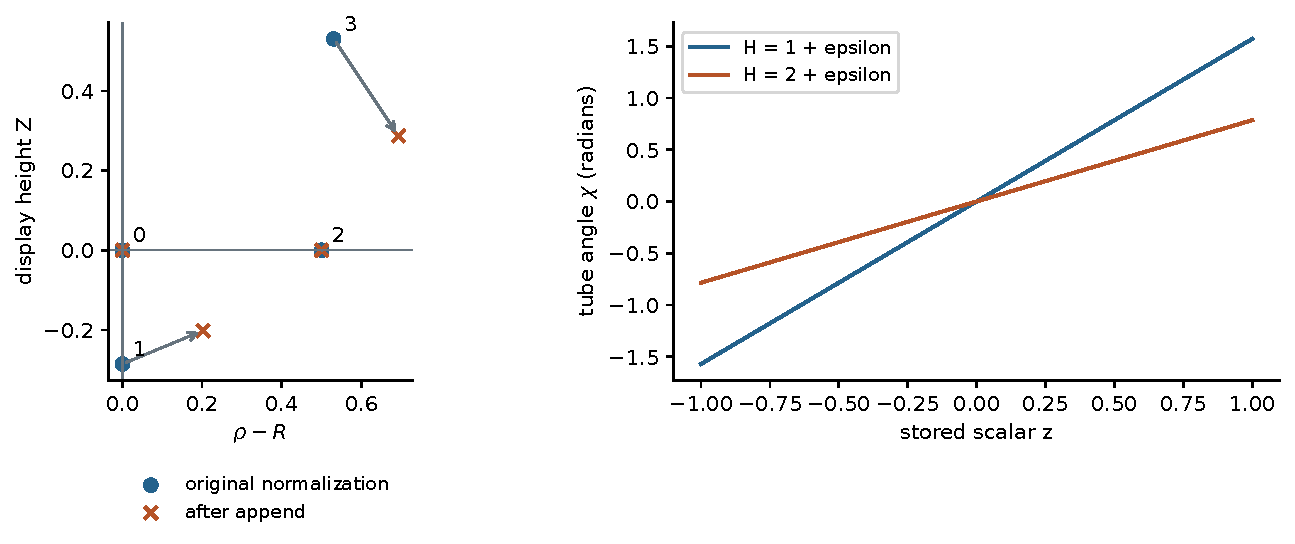
\includegraphics[width=\linewidth]{figures/history.pdf}
\caption{A history display in tube-plane coordinates
$(\rho-R,Z)$, which remove only the known azimuth.
With $R=2,r_{\max}=1,M=12$, histories share
$\kappa=(0,0.4,1,3)$, $q=(0,1,4,7)$,
$z=(0.6,-1,0,0.5)$. Adding a row $(1,2,2)$ changes the
normalization from $1+10^{-9}$ to $2+10^{-9}$.
Arrows connect the earlier points before and after this
change. The zero-radius row and the zero-scalar row stay fixed.
The right panel displays the two scalar-to-angle rules.}
\label{fig:history}
\end{figure}

\subsection{Cylinder and direct vectors}
For the same scalar and clock inputs the cylinder display is
\begin{equation}
 (X,Y,Z)=(\kappa\cos\vartheta,\kappa\sin\vartheta,z).
 \label{eq:cylinder}
\end{equation}
For $\kappa>0$ its inverse gives
$\kappa=\sqrt{X^2+Y^2}$, $\vartheta=\atan(Y,X)$ modulo
$2\pi$, and $z=Z$. At $\kappa=0$ it retains the scalar height,
but every admissible clock residue maps to $(0,0,z)$. The
azimuthal loss is nontrivial when $M>1$; with $M=1$ there was
only one residue. This is the opposite zero-radius scalar
behavior from \eqref{eq:history}.

Direct-vector extraction copies the three components of a
selected recorded vector. In the native source the default key
is \texttt{Z\_total}, with \texttt{Z\_vec} used only when that
default is absent \cite{diagnostics}. The map is an identity on
the selected vectors in their existing frame. This fact alone
does not make it injective on an unspecified complete state.
One would need a definition of that state and of its observation
map to ask the larger inversion question.

\subsection{A labelled logarithmic channel map}
The historical three-channel viewer uses fixed anchors
$\phi_j=0,2\pi/3,4\pi/3$ \cite{viewer}. Analyze one retained
label $j$ in its known Cartesian frame. For $R>r_0>0$, $c>0$,
and a nonzero complex input $\Omega$, set
\begin{equation}
 \rho_c=r_0[1+c\log(1+|\Omega|)],\qquad
 \theta=\arg\Omega\pmod{2\pi},
 \label{eq:channelradius}
\end{equation}
and
\begin{equation}
 (X,Y,Z)=
 \bigl((R+\rho_c\cos\theta)\cos\phi_j,\,
       (R+\rho_c\cos\theta)\sin\phi_j,\,
        \rho_c\sin\theta\bigr).
 \label{eq:channel}
\end{equation}
The subscript on $\rho_c$ distinguishes this tube radius from
the nonnegative spatial cylindrical radius. Its logarithmic
growth is unbounded. The original numeric formula implicitly
uses a dimensionless or already scaled modulus inside
$\log(1+|\Omega|)$.

\begin{proposition}[Labelled inverse and axis crossing]
\label{prop:channel}
For a point in the admitted image, retain the signed anchor
projection
\[
 u=X\cos\phi_j+Y\sin\phi_j.
 \]
Then
\begin{align}
 \rho_c&=\sqrt{(u-R)^2+Z^2},&
 m&=\exp\left(\frac{\rho_c/r_0-1}{c}\right)-1,\notag\\
 \Omega&=m\,\frac{u-R+\ii Z}{\rho_c}. \label{eq:channelinverse}
\end{align}
For nonzero input this is an exact inverse. A zero input is
recovered as zero from its conventionally chosen image; no
intrinsic argument for zero is required.
Negative signed projection occurs exactly when
$\rho_c>R$ and $\cos\theta<-R/\rho_c$.
\end{proposition}
\begin{proof}
Since the anchor vector is a unit vector, \eqref{eq:channel}
gives $u=R+\rho_c\cos\theta$, including when $u<0$.
The norm of $(u-R,Z)$ recovers $\rho_c\geq r_0>0$.
Inverting the logarithm gives $m=|\Omega|$, and division by
$\rho_c$ recovers $\cos\theta+\ii\sin\theta$. Their product
is $\Omega$. At zero, $m=0$, so that product recovers zero
for any explicitly chosen forward angle convention. The
historical numeric routine uses its library's zero-angle
convention; the complex number zero itself has no argument.
Finally $u<0$ is exactly $R+\rho_c\cos\theta<0$, giving the
stated pair of conditions.
\end{proof}

The label matters: replacing $u$ by $\sqrt{X^2+Y^2}=|u|$
folds the negative branch and invalidates this inverse.
At the shared axis different labels also lose their distinct
anchor directions. Without the label, the union of channels
need not be injective. With the label retained, the signed
inverse remains valid at an axis point.

Large modulus \emph{permits} crossing when
$|\Omega|>\exp((R/r_0-1)/c)-1$, but does not force it;
phase $\theta=0$ always gives positive $u$.
The visual background wireframe has fixed tube radius $r_0$.
It is not the surface carrying all the channel points.

\par\noindent\begin{minipage}{\linewidth}
\begin{proposition}[Nonzero re-entry into the background wireframe]
\label{prop:reentry}
Let the background ring be
\[
 W=\{(X,Y,Z):(\sqrt{X^2+Y^2}-R)^2+Z^2=r_0^2\}.
 \]
On the branch $u\geq0$, a channel point lies on $W$ only for
$|\Omega|=0$. On the branch $u<0$, it lies on $W$ precisely
when
\begin{equation}
 2R-r_0\leq\rho_c\leq2R+r_0,\qquad
 \cos\theta=\frac{r_0^2-4R^2-\rho_c^2}{4R\rho_c}.
 \label{eq:reentry}
\end{equation}
Thus the admissible nonzero modulus band is
\begin{equation}
 \exp\left(\frac{2R/r_0-2}{c}\right)-1
 \ \leq |\Omega|\leq\
 \exp\left(\frac{2R/r_0}{c}\right)-1,
 \label{eq:reentryband}
\end{equation}
with the phase condition in \eqref{eq:reentry} still necessary.
\end{proposition}
\end{minipage}\par
\begin{proof}
The cylindrical radius of a channel point is $|u|$. If
$u\geq0$, its squared distance from the background meridian
centre is $(u-R)^2+Z^2=\rho_c^2$, which equals $r_0^2$
only for $\rho_c=r_0$, hence $|\Omega|=0$.

If $u<0$, using $|u|=-u$ gives
\[
 (|u|-R)^2+Z^2
 =\rho_c^2+4R\rho_c\cos\theta+4R^2.
 \]
Equating this to $r_0^2$ gives the cosine in
\eqref{eq:reentry}. That cosine is at most $1$ automatically,
because $r_0<R$ and its numerator is negative. It is at
least $-1$ exactly when
$(\rho_c-2R)^2\leq r_0^2$, proving the radius band.
On that band $\rho_c\geq2R-r_0>r_0$, and substitution yields
$u=(r_0^2-\rho_c^2)/(4R)<0$, so the branch condition is
indeed satisfied. Monotonic inversion of
\eqref{eq:channelradius} gives \eqref{eq:reentryband}.
\end{proof}

At the historical defaults $R=2,r_0=3/5,c=2/5$, choose
\begin{equation}
 \Omega=-\bigl(\exp(35/3)-1\bigr),\qquad \phi_j=0.
 \label{eq:channelwitness}
\end{equation}
Then $\theta=\pi$, $\rho_c=17/5$, and the point is
$(-7/5,0,0)$, which lies on $W$ since
$(7/5-2)^2=9/25=r_0^2$. This nonzero witness prevents the
incorrect assertion that only a zero channel can ever meet
the background. The upper endpoint of the modulus band is
$\exp(50/3)-1$. These are properties of the display map;
they do not establish that a native trajectory reaches these
inputs.

\begin{figure}[tb]
\centering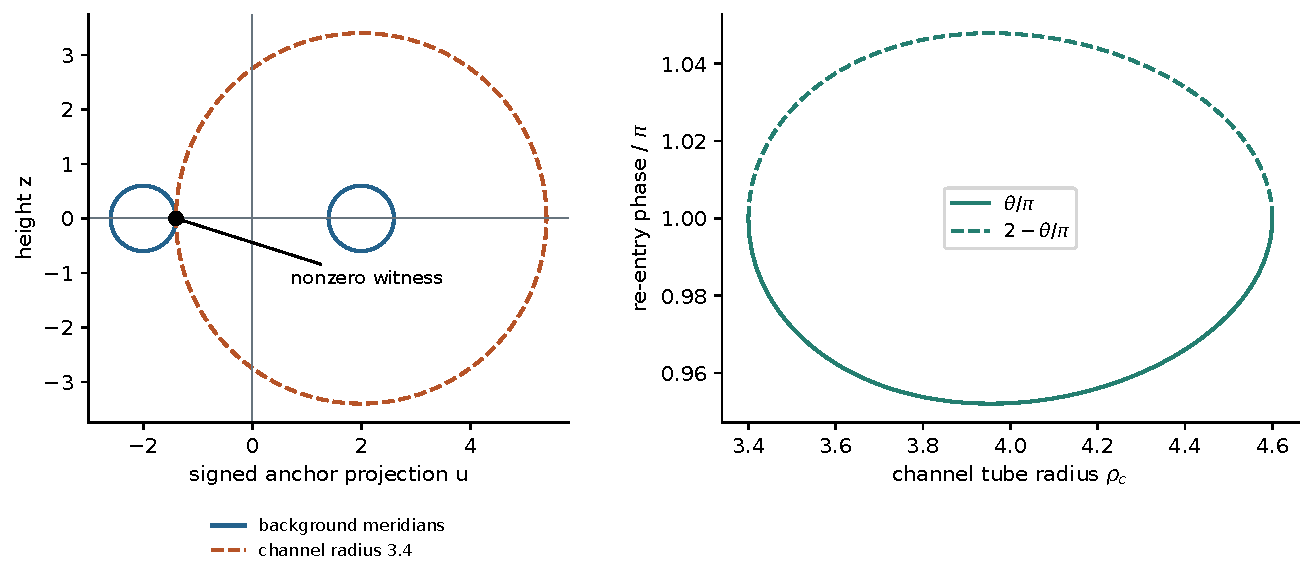
\includegraphics[width=\linewidth]{figures/channel.pdf}
\caption{Labelled channel geometry at $R=2,r_0=0.6,c=0.4$,
$\phi_j=0$. Left: the signed anchor plane $(u,Z)$ shows the
two background meridian circles and the tube-radius
$\rho_c=3.4$ locus (dashed); the nonzero witness is
$(-1.4,0)$. Right: the allowed negative-branch re-entry
phases over $3.4\leq\rho_c\leq4.6$. A radius in this band
alone does not put a point on the wireframe.}
\label{fig:channel}
\end{figure}

\subsection{Exact inverses and finite precision}
Exact branch and side-information conditions are part of
each theorem. Floating arithmetic can round
$\kappa/(1+\kappa)$ to one, round $H_z$ to the maximum
despite the positive regularizer, or lose accuracy in
$\rho-R$. A successful finite floating result therefore does
not certify the strict inequalities used by
Theorem~\ref{thm:history}. The native routine's documentation
explicitly warns about such saturation \cite{diagnostics}.
The channel exponential can also overflow for large decoded
radii. These cautions limit numerical use of the formulas;
they do not alter the exact fibres proved above. We have not
implemented or certified a runtime inverse.

Colour and percentile displays introduce additional
normalization or clipping, summarized in
Appendix~\ref{app:display}. They require their own retained
scale and frame information. A coordinate loss in one map
must not be generalized to all stored records or to a
different display.

\section{Consequences and limits}
\label{sec:conclusion}
The full-image intersection interval, strict spindle-body
containment, and the exact shared witness answer different
geometric questions. A homothetic chart family can have
intersecting spindle images while its diagnostic bodies are
strictly nested. The positive result is a precise
classification, rather than a single ambiguous claim about
overlap.

The prescribed common-angle sum yields an equally concrete
observation law: three real coefficient functions determine
its entire phase-indexed squared modulus. Three suitable
known samples recover these coefficients; complex amplitudes
and individual shell weights require other information.
The restricted rigid-rotation theorem then uses the actual
azimuthal dependence, not the appearance of selected plots.

Measures and displays complete the information accounting.
Normalization is conditional on a chosen measure and a
positive integral. An ambient extension can be constructed,
but is not uniquely determined by its restriction. A
history-torus XYZ record, its richer retained record, a
cylinder, and a labelled logarithmic channel have different
exceptional fibres. These distinctions are sufficient to
describe the defined mathematics without assigning any of
the objects a physical field interpretation.

\appendix
\section{Bounded source correspondence}
\label{app:sources}
The primary equations for the radii, chart, Gaussian weights,
phase sum and squared modulus occur in
\emph{Converging Symmetries}, version dated 27 May 2025,
physical pages 1--2, Eqs.~1--8 \cite{cs1}. The source's
Gaussian-centre notation is unindexed $R$; we use $C$ to
avoid identifying it with the unscaled radius parameter $R_*$.
The historical source denotes that parameter by $R_0$; here
$R_*$ distinguishes it from the indexed zeroth radius
$R_{n=0}=\bar R$. This notation change preserves the radii.
A later version dated
28 May 2025 has a different printed author line \cite{cs2}.
The title, date and supplied edition are retained in the
source ledger; it is not silently treated as the same
bibliographic item.
The later recursive-field paper reproduces the scaled
construction on physical page 17, Sec.~19.1,
Eqs.~18--19 \cite{rt}. Its presentation does not by itself
supply a map from the common-angle scalar observation to a
spatial field with an evolution equation.

The visually confirmed physical page 4 of that paper contains
two further, distinct prescriptions \cite{pageSupplement}.
In Sec.~3.1 the curve family is
\begin{equation}
 x=(R+0.1i)\cos t,\quad y=(R+0.1i)\sin t,\quad
 z=0.2(1-0.15i)\sin2t.
 \label{eq:rtcurve1}
\end{equation}
Here $i$ is a curve index, not the imaginary unit $\ii$;
its range is not specified in that prescription.
Section~3.2 gives code for five curves $i=0,\ldots,4$,
with 200 equally spaced $t$ values from $0$ to $2\pi$ and
\begin{align}
 \delta&=0.1\sin(5t+i),\notag\\
 x&=(R+r\cos(t+i)+\delta)\cos t,\notag\\
 y&=(R+r\cos(t+i)+\delta)\sin t,\qquad
 z=r\sin(t+i).
 \label{eq:rtcurve2}
\end{align}
These are prescribed curves, not the sum \eqref{eq:psi}.
For the continuous expression \eqref{eq:rtcurve2}, take
$i=0,t=\pi/2$, with $R,r>0$. It gives
$(0,R+0.1,r)$, whose squared meridian distance from the
unperturbed torus core is $r^2+0.01$, not $r^2$.
This exact witness concerns the formula; it need not be
one of the 200 sampled points.

The historical file \texttt{recursive\_field\_evolve.py}
does contain an actual coordinate-update algorithm
\cite{fieldCode}. Its \texttt{evolve\_field} constructs
five-nearest-neighbor adjacency, uses a mean neighbor
displacement and its componentwise hyperbolic tangent,
adds a centre-directed bias and random perturbation, and
applies a step-dependent multiplier to the third coordinate.
The adjacency is constructed before the step loop. Some
named constants and the computed breathing amplitude do not
enter the coordinate update. These facts follow from text
inspection, not execution. No explicit source map identifies
this algorithm with \eqref{eq:psi}, its extension, or a
native computational shell.

The native and historical coordinate adapters are separate
sources for Section~\ref{sec:displays}
\cite{diagnostics,geometry,viewer}. A historical fixed
12-sector angle and the native modular clock agree for
integer clock inputs at that clock size. Their source lineage
does not turn the Gaussian carrier family into the input
state of the display.

The remaining historical gaps are narrow: definitions and
domains of the recursive operators denoted $G,T$; a specified
norm or metric and field type for related operator claims;
a measure and numerical threshold for the historical
intensity display; and a transport or consumer map joining
the distinct constructions. A time-only seed does not
exclude unknown operators introducing spatial dependence.
Likewise a scalar expression does not supply a vector curl
without a declared vector-valued reading. These missing
definitions are recorded, not completed by conjecture.
The page-4 confirmation and received final addendum are
closed evidence items, not current gaps.

\section{Colour and percentile transformations}
\label{app:display}
The viewer's trail colour uses
$(J-J_{\min})/(J_{\max}-J_{\min})$ when the range is
positive, and zero for a constant series
\cite[lines 419--424]{viewer}. Even before a colour map,
the normalized values need the extrema to recover the
original scale. The constant branch collapses every
constant level to zero unless that level is retained.
A displayed RGB value additionally depends on the colour
map and its possible quantization; it is not assumed to
be an exact inverse code for a scalar.

A different spectral display floors energies at $10^{-12}$,
takes their logarithms and then applies range normalization;
it uses a separate clipped brightness factor
\cite[lines 537--549]{viewer}. All values below the floor
have the same transformed energy. Retaining extrema can
invert a nonconstant logarithmic range above the floor,
but cannot undo the floor itself. Retaining a coordinate
array also does not undo a clipped colour channel.

The vector overlay uses the $99$th percentile $d$ of finite
vector norms greater than $10^{-12}$, and multiplies the
selected vectors by $0.85r_{\mathrm{frame}}/d$
\cite[lines 652--665]{viewer}. When that selection is empty,
or the resulting denominator is nonfinite or at most
$10^{-12}$, the code uses $d=1$. Recovering an input vector
from a scaled plotted vector requires the actual scale and
frame; selecting one vector array is still not a definition
of a complete state. These transformations are reported
individually rather than combined into a global claim that
all display coordinates lose the same information.

\section{Reproducibility, attribution, and review status}
\label{app:repro}
The accompanying supplement contains the editable source,
bibliography, six reproducible figures and their declared
numeric data, one isolated checker, exact command records,
compiler logs, and a page-by-page visual receipt. The
generators are collected in one script. Checks transcribe
the mathematical definitions independently; they do not
import or execute the project runtime or replay earlier
research suites. Exact symbolic identities, exact witnesses,
and finite numerical illustrations are distinguished in
the results. The analytic proofs of theorems, particularly
Theorem~\ref{thm:rotation}, do not depend on a finite
test count.

The proofs apply classical tools to the stated family.
The body $K_n$, the extension family, and the selected
figure parameters are declared mathematical constructions.
The spindle and wireframe examples are counterexamples
to broader identifications, not historical measurements.
The accompanying proof/source/literature inventory records
these roles. Literature checking is targeted, with no claim
of comprehensive novelty clearance.

Hilmir Frímann Halldórsson is the sole named author of this
manuscript. Codex prepared the draft and this revision, its derivations,
figures, checks and typesetting under the owner's work
order. GPT supplied scientific reconciliation and accepted
qualifications. Claude contributed an independent prior
research pass and the received reconciliation addendum;
that prior work is not a review of this manuscript.
Some historical sources explicitly credit GPT or ChatGPT
in their printed author lines, retained in the bibliography.

Version 0.1 received a GPT manuscript review and a Codex
author re-review. Codex also drafted that edition; its
re-review is not an independent Claude manuscript review,
regardless of the retained legacy report filename. Claude's
earlier independent research pass and reconciliation addendum
remain distinct from manuscript review. No external peer
review or journal acceptance is claimed.

This v0.1.1 repository-research candidate applies the accepted
radius-notation and phase-wording corrections and updates
this review account. Final GPT verification of these revised
bytes and confirmation of the exact public payload remain
pending. The separate lens v0.1.1 edition retains its accepted
bytes. No publication or release has occurred in this task,
and no new licence is selected.

\bibliographystyle{plain}
\begingroup\raggedright
\bibliography{references}
\endgroup
\end{document}
